\section{Introduction}
\label{sec:intro}

% Semantic segmentation and MIC
At its core, semantic segmentation is tasked with associating pixels, or voxels, of an image with a label that corresponds to a meaningful category. As a fundamental problem in medical image computing, an impressive amount of research on the topic has been conducted in recent years, spanning methods that segment tumors in MRI volumes \cite{zikic2014,menze15}, airways from chest CT scans \cite{miyawaki17}, vessels in retinal scans \cite{pilch12} or mitochondria in electron microscopes \cite{seyed13} to name a few.

% Machine Learning and semantic segmentation
To this day, the vast majority of state-of-the-art segmentation approaches rely heavily on supervised machine learning frameworks \cite{sweeney14,menze15}, and in particular deep learning \cite{garcia17}, to produce excellent segmentation results. In general, these methods depend on large amounts of training examples to learn complex prediction models. Critically, most of these models are trained using pixel-wise annotations associated with training examples. While highly effective, the cost of acquiring such pixel-wise annotations for training machine learning methods is often overlooked and yet a central limiting factor for aggregating extremely large training datasets. This is particularly the case for video and 3D image data where annotations are extremely costly (\ie days per video sequence). This in turn negatively impacts the capacity to train high-performing segmentation models, as the number of training samples remains relatively small.

% General statement about semi-supervised learning.
To reduce the burden of producing pixel-wise annotations, a number of semi-supervised concepts have been proposed such as active learning \cite{KonSznFua15}, domain adaption \cite{tzeng17} and crowd-sourcing \cite{mavandadi12}. Alternatively, a number of recent methods propose to infer pixel-wise segmentation directly from image labels (\ie the image contains a tumor) by leveraging strong object or shape priors \cite{menze10}. In effect these methods attempt to refine segmentations from pre-trained neural networks for generic object classes \cite{su15} or trained attention models \cite{kingma14}. While extremely promising, such methods still only produce coarse segmentations and remain ill suited for training complex prediction models.

% Impact of input type
At the same time, the method by which annotations are provided has important practical implications in terms of convenience for the annotator and can also greatly speed-up the annotation process \cite{ferreira12}. For example, providing tumor pixel segmentations in volumetric data would be infeasible if each pixel were to be specified individually. Instead, there is an important body of work that has considered alternative user-interaction mechanisms. For instance, \cite{KonSznFua15} used 3D image planes to specify the boundary between image backgrounds and objects in 3D modalities. Scribbles of positive and negative image regions were also shown to be effective in speeding up annotation generation \cite{roberts11}. Even more efficient, was the use of 2D points to sparsely annotate image data \cite{bromiley14,bearman16}. Such 2D point supervision is interesting as it can be produced by manually clicking on images from 3D volumes or video sequences, or by using a gaze tracker to passively record 2D coordinates of the object as they are viewed \cite{yunpeng13,khosravan16,lejeune17}. This latter strategy is promising as it holds the potential to annotate at high framerate, but is challenging due to limited, if any, information regarding the background. To overcome this, previous methods that generate segmentations from 2D supervision have relied on strong assumptions on the object size, the background scene, or clouds of 2D locations, whereby limiting usability.

To generalize the use of sparse 2D point supervision to infer segmentations in a given image volume or sequence, we propose a novel framework that avoids the need to assume much about the object and only requires 2D object locations to be specified. In particular, we assume that the object of interest is compact and always present in the image, but can have arbitrary size regardless of the image modality considered. With the goal of segmenting this object of interest, our method first builds an object appearance model from the provided 2D locations. We then construct a 3D graph over the entire image data, from which the complete object segmentation is estimated in each frame. To do this, the graph is optimized in a multi-source, single sink max-flow setting that uses the object model and we show that this problem can be solved optimally using a K-shortest path approach. We then iterate this optimization procedure using the previously obtained result to update our object model and thus refine the produced segmentations. In order to achieve consistent segmentations from such sparse annotations regardless of the image type or object, we also propose to use image and object specific features that are learned from the image data. This is achieved by using a Convolutional Neural Network (CNN) and a novel loss function that takes into account the 2D image locations. Combined, we show that our framework provides a significant improvement over existing methods on a number of varied datasets (see Fig.~\ref{fig:fig1}). We show that our results are not only more similar to traditional hand segmentations to those produced by state-of-the-art methods, but that they only induce mild reductions in performance when used to train prediction models. Beyond this, we show that by using a low-cost gaze tracker to generate supervised 2D locations, a user can generate annotations at high framerate.

\begin{figure}[t!]
\centering
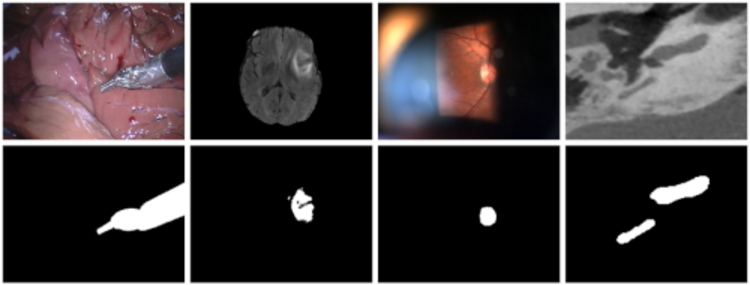
\includegraphics[width=0.99\textwidth]{fig1.pdf}
\caption{Example of objects of interest in different video and volumetric modalities. The bottom row shows the pixel wise segmentation for each case: From left to right: A surgical instrument during an endoscopic procedure, a 3D MRI scan containing a brain tumor, an optic disc seen from a slit lamp microscope and a cochlea cross-section in a 3D CT scan.}
\label{fig:fig1}
\end{figure}
 
In the following sections, we begin by describing existing methods closest to our work. We then introduce our framework in Sec.~\ref{sec:overview} and describe its detail thereafter. In Sec.~\ref{sec:results}, we show how our method performs on a number of tasks and datasets, as well as compared to existing methods.

%%% Local Variables:
%%% mode: latex
%%% TeX-master: "../../main"
%%% End:
